\subsubsection{La estructura temporal de la conciencia del ahora: impresión originaria, retención y protención}\label{sec:estructura-tripartita}

Sin ir más lejos, pasemos a examinar la estructura tripartita inmanente
de la conciencia del ahora: la impresión originaria, la retención y la
protención con los momentos correlativos captados en estas: el ahora
puntual, el ahora-reciente y el ahora-adveniente: `` \ldots Sobre
cada `ahora' es la estructura `protoimpresión-retención-protención' de
la conciencia absoluta la que articula el darse de lo temporal. Esta
opera como una estructura invariante'' \cite[p.~251]{kretschel2014}. La mirada
natural del tiempo objetivo presupone este desdoblamiento de la
temporalidad consciente, lo que quiere decir que todo presente marcado
por el tiempo objetivo necesita darse en el horizonte de un antes y
después. Para yo saber que dar una vuelta por el parque con mi mascota
me toma de las 11:30 hasta las 12:00, es decir, para poder trazar una
secuencia de tiempo objetivo, implícitamente debo captar un horizonte de
momentos pasados y futuros a partir del instante actualmente marcado
objetivamente. Condición de posibilidad para captar y delimitar el lapso
temporal de los sucesos espacializados es que la propia conciencia ya es
una duración temporal de vivencias de dichos objetos. Sólo porque dichas
vivencias poseen una duración temporal en la cual fenomenológicamente se
pueden distinguir las fases que marcan las direcciones temporales de
presente, pasado y futuro, es que se puede comprender la sucesión de
momentos de tiempo objetivo. Pero este, al nivelar todos los instantes
como una serie de puntos homogéneos, no puede captar la distinción
esencial de temporalidad inmanente entre ellos.

Es necesario notar que la estructura del tiempo inmanente de la
conciencia no se da en el tiempo objetivable en el modo en que se dan
nuestras vivencias particulares, ya que esto nos llevaría a una
regresión infinita \cite[p.~86]{zahavi2010}\footnote{Esto quiere decir que el
  acto mismo debe de poseer ciertas estructuras que condicionen toda
  vivencia presente, pasada y futura, posibilitando que la conciencia
  pueda volver a ellos reflexivamente por su continuidad temporal. La
  conciencia no solo trasciende hacia objetos externos a ella, sino que
  puede reconducir su ``mirada'' hacia sus mismos actos y examinarlos
  aunque no con el mismo sentido de objetividad: podemos volvernos hacia
  todo acto en el horizonte temporal de la vida consciente. Todo acto de
  la conciencia posee la posibilidad de ser reflexivo, es decir, de
  poder volver sobre mis propias vivencias. Esto es característico de
  los actos noéticos y marca un contraste con los objetos dados. Por
  dicha estructura temporal de la conciencia, se muestran los diferentes
  niveles del acto consciente que entran en juego en toda vivencia
  intencional y que unifican en toda experiencia vivida la temporalidad
  de la conciencia con la temporalidad objetiva. ``La afirmación no es
  que el objeto de experiencia siempre debe diferir ontológicamente del
  sujeto de experiencia, como si el sujeto y el objeto de experiencia
  debieran ser necesariamente dos entidades diferentes. Más bien, la
  afirmación es simplemente que la experiencia en sí misma no se
  experimenta de forma prerreflexiva como un objeto \ldots. Lo que
  esto significa, sin embargo, es que sería un error concebir la
  relación entre la conciencia interna del tiempo y la experiencia
  intencional como si fuera una relación objetivante entre dos
  dimensiones distintas de la conciencia'' \cite[p.~332]{zahavi2010}.}. La
estructura temporal de la conciencia es lo que nos permite captar el
devenir temporal de nuestras vivencias y, por lo tanto, ella misma no
puede estar sometida a dicho devenir. No hay instancia anterior a ella
para captar el devenir temporal y, por lo tanto, todo análisis
fenomenológico del tiempo supone dicha estructura para que sea posible
la captación de una vivencia en general. El tiempo como ``algo''
distinguible la conciencia no es comprensible dentro de un análisis
fenomenológico: el tiempo se da en el terreno de la vida consciente.
Separar la estructura esencial de la conciencia del ahora de la
temporalidad objetivada es necesario para comprender la posibilidad de
la reflexión sobre las vivencias. Si bien las vivencias se pueden
objetivar al reflexionar sobre ellas, eso no significa que \emph{sean}
objetos o que aparezcan inicialmente como objetos, sino que, en tanto
\emph{vivencias,} se manifiestan en primera instancia como \emph{vividas
desde mí} e in-objetivables como cosas \emph{dadas}, pero \emph{pueden
volverse} objetos de la conciencia si es que esta se vuelve a ellas a
partir de un acto reflexivo que surge en su horizonte temporal. Esta
distinción fenomenológica evita una bifurcación ontológica radical entre
la vivencia y el objeto dado, ya que la vivencia no es un objeto como
los objetos intencionales dados en ellas, sino que se objetiva en el
mismo horizonte temporal en el que fue dada. Para poder reflexionar
sobre la estructura temporal de mis propias vivencias, no necesito
suspender el discurrir temporal mismo, sino distinguir, en él, las fases
esenciales intrínsecas a toda vivencia.

Husserl caracteriza a las vivencias examinadas en su duración temporal
como ``fenómenos decursivos'', ya que captamos la continuidad de
constantes mudanzas que ``forma una unidad inseparable; inseparable en
trechos que pudiesen existir por sí, e indivisible en fases que pudiesen
existir por sí, puntos de la continuidad'' \cite[§10, p.~50]{husserl2002}. Al
dirigir nuestra mirada a las vivencias en su duración temporal, lo que
captamos es un curso continuo de mudanzas que contienen captados a los
instantes puntuales del tiempo objetivo que medimos en la actitud
natural. Por eso, ``los fragmentos que nosotros abstractamente
destacamos sólo pueden existir en el decurso íntegro, y lo mismo las
fases, los puntos de la continuidad decursiva'' (Husserl, 2010, §10,
50). En otras palabras, la condición de posibilidad de toda captación de
tiempo, ya sea cuando contamos el tiempo objetivo del reloj o cuando
subjetivamente percibimos su paso, es captar una duración unitaria que,
al examinarla, nos muestra un tránsito constante de fases temporales que
indican las direcciones de pasado, presente y futuro. Antes de cualquier
referencia objetiva o subjetiva al tiempo, hay una estructura esencial
de duración temporal operando en toda vivencia consciente. Si bien estas
fases muestran el discurrir constante de la duración temporal, ``podemos
decir con evidencia que es en cierto modo inmutable en su forma''
\cite[§10, p.~50]{husserl2002}. Husserl busca notar el doble carácter de
multiplicidad y unidad del examen de la duración temporal de las
vivencias conscientes: por un lado, es una sola duración que captamos,
pero en dicha duración se muestra un discurrir constante de fases
temporales que es invariable en su estructura esencial de impresión
originaria-retención-protención que, por lo tanto, no está sometida ella
misma a un devenir temporal, sino que se mantiene invariable en toda
vivencia examinada.

En ese sentido, la conciencia puede captar su temporalidad volviéndose
sobre sus propios actos y las estructuras que lo condicionan separando
dicho análisis del objeto dado en las vivencias. Es esta estructura
temporal de la conciencia del ahora la que posibilita el sentido de lo
pasado, presente y futuro en la continuidad de la vida consciente y que
el tiempo objetivo supone en la sucesión de instantes. Ahora, pasemos a
examinar el gráfico que presenta Husserl en el parágrafo 10 de las
\emph{Lecciones}\footnote{Husserl, 2002, §10, 50.}:

\begin{figure}[htbp]
    \centering
    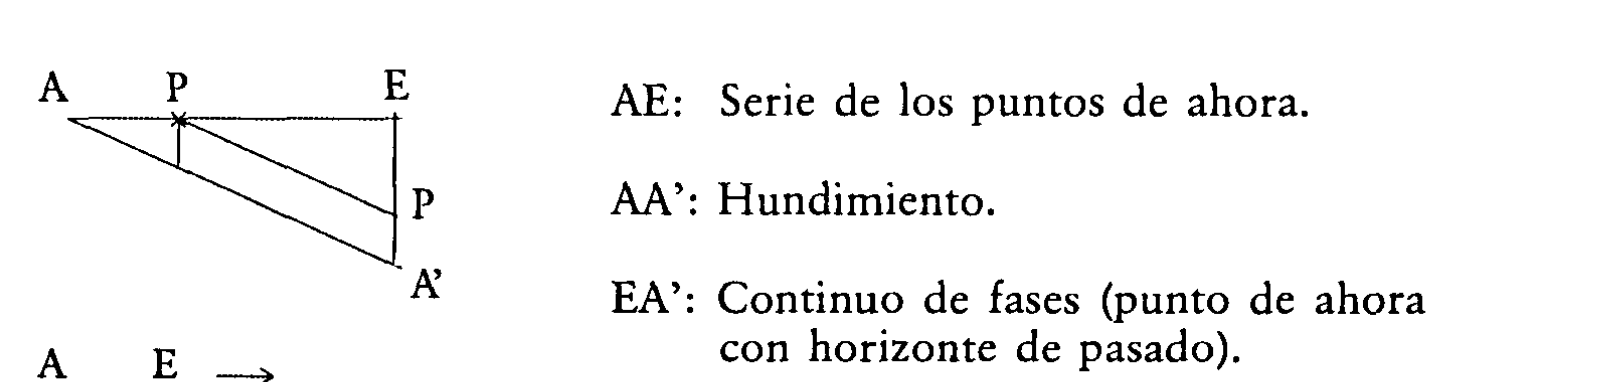
\includegraphics[width=0.88\textwidth]{figuras/diagrama_husserl_original.png}
    \caption{Diagrama de la conciencia interna del tiempo presentado por Husserl en el §10 de las \textit{Lecciones}.}
    \label{fig:diagrama-husserl}
\end{figure}

Husserl no desconoce la puntualidad irreductible del ahora. Este
carácter puntual es lo que denominamos ``instante'' en referencia al
tiempo objetivo y que en la conciencia interna del tiempo corresponde
directamente a un momento abstracto de la fase o duración. Lo que
permite la descripción de la duración de la conciencia del ahora es
comprender la estructura que permite la captación temporal de toda
vivencia en sus fases de impresión originaria-retención-protención. La
línea horizontal marca esta serie de \emph{ahoras} puntuales (AE)
captada como una continuidad constante. Estos, claramente, no se dan
simultáneamente, sino que se caracterizan por una continuidad que forma
la duración temporal. Asimismo, como vemos, esta no es una línea
horizontal, sino que posee puntos verticales que indican el hundimiento
de los puntos retenidos en el punto actual, lo cual muestra que la
duración temporal de la conciencia del ahora posee una profundidad
formada por los puntos temporales dejados atrás. El punto A no
desaparece, sino que se va hundiendo hasta ser un A', es decir, que es
retenido en el punto E a medida que el ahora sigue discurriendo y que
permanece constante en todo punto adveniente. Esta transformación del
ahora puntual a partir de una continuidad de momentos re-tenidos y
pro-tenidos, de ahoras recientes y ahoras advenientes estructura la
conciencia interna del tiempo.